%Configuração das fontes e formato
\documentclass[12pt,a4paper,notitlepage]{report}
\usepackage[utf8]{inputenc}
\usepackage[brazilian]{babel}
\usepackage[T1]{fontenc}
\usepackage{tgpagella}
\usepackage[final,protrusion=true,expansion]{microtype}
\usepackage{indentfirst}

%Pacotes para que equações matemáticas fiquem melhores
\usepackage{amsmath}
\usepackage{amsfonts}
\usepackage{amssymb}

%Pacotes de cores e lidar com imagens
\usepackage{graphicx}
\DeclareGraphicsExtensions{.pdf,.eps,.png,.jpg}
\usepackage{xcolor}
\definecolor{dkgreen}{rgb}{0,0.6,0}
\definecolor{gray}{rgb}{0.5,0.5,0.5}
\definecolor{mauve}{rgb}{0.58,0,0.82}

%Evitar linhas soltas no topo da página
\usepackage[all]{nowidow}

%Mais opções de personalização ao fazer o enumerate, itemize
\usepackage{enumitem}

%Tirar margem das listas
\setlist[itemize]{leftmargin=*}
\setlist[enumerate]{leftmargin=*}
\setlist[description]{leftmargin=*}

%Criação de cronogramas/etc
\usepackage{pgfgantt}

%Unidades do SI e formatos de colocar valores numéricos
\usepackage{siunitx}

%Controlar a tipografia do sumário e lista de figuras
\usepackage{tocloft}

%Deixas as imagens no local correto
%Usar [H]
\usepackage{dblfloatfix}
\usepackage{float}

%Citações
%\usepackage[alf]{abntex2cite}
\usepackage{natbib}

%Colocar código no documento
\usepackage{listings}
\lstset{frame=tb,
   language=[Sharp]C, %C#
   aboveskip=3mm,
   belowskip=3mm,
   showstringspaces=false,
   columns=flexible,
   basicstyle={\small\ttfamily},
   numbers=left,
   numberstyle=\tiny\color{gray},
   keywordstyle=\color{blue},
   commentstyle=\color{dkgreen},
   stringstyle=\color{mauve},
   breaklines=true,
   breakatwhitespace=true
   tabsize=3
   }

%Deixar PDF com título e autor
\usepackage[breaklinks]{hyperref}
\hypersetup{
%     bookmarks=true,
    pdftitle={Padrão de Relatórios \the\year},
    pdfauthor={Jonathan Gouvea da Silva},
    hidelinks
}

% Formato das seções e sumário
\setcounter{tocdepth}{4}
\setcounter{secnumdepth}{4}
\renewcommand{\thesection}{\arabic{section}}
\renewcommand{\thesubsection}{\arabic{section}.\arabic{subsection}}
\renewcommand{\thesubsubsection}{\arabic{section}.\arabic{subsection}.\arabic{subsubsection}}

%Tamanho do parágrafo e identatação
\setlength{\parindent}{4em}
\renewcommand{\baselinestretch}{1.5}

\title{Padrão de relatórios}
\author{Jonathan Gouvea da Silva}
\date{September 2018}

%%%%%%%%%%%%%%%%%%%%%%%%%%%%%%%%%%%%%%%%%%%%%%%%%%%%%%%%%%

\begin{document}

\makeatletter
\begin{titlepage}
	\centering
	{\normalsize Universidade Federal de São Carlos\\Centro de Ciências Exatas e de Tecnologia\\Departamento de Computação}
    
	\vspace{4cm}
    {\LARGE \@title}
    
    \vspace{1em}
	{\normalsize Relatório}
    
    \vspace{5em}
    {\large Alunos\\}
    {\normalsize \@author}
    
    \vspace{4em}
    {\large Professor\\}
    {\normalsize Prof. Dr. }
	
    \vfill
    {\normalsize \@date}
\end{titlepage}
\makeatother

\tableofcontents
\clearpage
\listoffigures
\clearpage


\section{Introduction}
There is a theory which states that if ever anyone discovers exactly what the Universe is for and why it is here, it will instantly disappear and be replaced by something even more bizarre and inexplicable.
There is another theory which states that this has already happened.

\begin{figure}[H]
\centering
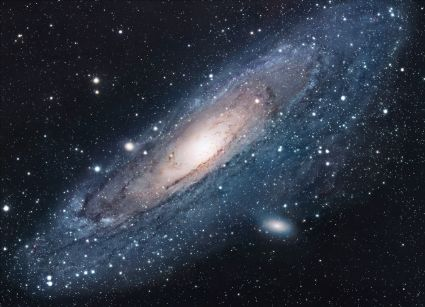
\includegraphics[scale=1.7]{universe}
\caption{The Universe}
\label{fig:universe}
\end{figure}

\section{Conclusion}
``I always thought something was fundamentally wrong with the universe'' \citep{adams1995hitchhiker}

\bibliographystyle{plain}
\bibliography{references}
\clearpage
\end{document}

